\section{Filtro pasabajos}

%TODO Aclarar lo de como se midio con x1 o x10 y por que

%TODO Unidades correctamente en todas las tablas
%TODO Redondear todas las mediciones

\subsection{An\'alisis te\'orico}

\subsubsection*{Modelos ideales}

Para el an\'alisis te\'orico del circuito se asume una condici\'on de idealidad en el generador de señales que se conecta en la entrada del circuito, y lo mismo se aplica para los componentes, pues no se consideran los efectos par\'asitos propios de las caracter\'isticas constructivas de los mismos.

\begin{figure}[H]
\centering
\begin{circuitikz}[american voltages]
		\tikzstyle{every node}=[font=\footnotesize]	
		\draw
		(0,-1) to[american voltage source, l=$v\left(t\right)$, invert] ++(0,2) -- ++(0.5,0)
		to[R, l=$R$, v=$v_r$, i=$i\left(t\right)$] ++(2,0) -- ++(0.5,0) node[]{}
		to[C, l=$C$, v=$v_c$] ++(0,-2)
		to[short, -*] ++ (-1.5,0) node[ground, scale=0.6]{} to[short] ++(-1.5,0);
\end{circuitikz}
\caption{Circuito te\'orico RC}
\end{figure}

Del circuito se busca la funci\'on de transferencia que vincula la excitaci\'on, señal del generador, y la tensi\'on de salida que ser\'ia la medida sobre el capacitor. 

\begin{equation}
	H(s) = \frac{V_c}{V} = \frac{\frac{1}{s \cdot C}}{\frac{1}{s \cdot C} + R} 
	= \frac{1}{1 + s \cdot R \cdot C}
	\label{eq:transfer}
\end{equation}

%TODO Agregar referencia al ploteo de la respuesta en frecuencia!

En la expresi\'on anterior, asumiendo que el circuito tiene un comportamiento LTI, causal y bibo-estable, se obtiene que la respuesta en frecuencia del circuito resulta de evaluar a la variable de frecuencia compleja en $s = j\omega$ y se obtiene:

\begin{equation}
	H(f) = \frac{1}{1+ j 2 \pi \cdot f \cdot R \cdot C}
\end{equation}
 
La funci\'on transferencia obtenida presenta un polo simple que ser\'a la frecuencia de corte, ubicada en $f_o = \frac{1}{2 \pi \cdot R \cdot C}$. Como se puede ver en la figura \ref{fig:bode_modulo} en la secci\'on de resultados, el comportamiento de tal circuito frente a la frecuencia es de un pasabajos, pues presenta una transferencia que aten\'ua las altas frecuencias. El valor caracter\'istico de la respuesta en frecuencia a la frecuencia de corte est\'a dado por:

\begin{equation}
	H(f_o) = \frac{1}{1 + j2 \pi f_o RC} = \frac{1}{\sqrt{2}} \phase{45^{ \circ}}
	\label{eq:condition}
\end{equation}

\subsubsection*{Modelo equivalente del capacitor}

En este apartado el an\'alisis te\'orico que se hace considera algunos de los efectos par\'asitos del capacitor, los cuales son tenidos en cuenta en su modelo equivalente incorporando, para la configuraci\'on paralelo, la resistencia interna que se atribuye a las p\'erdidas en el diel\'ectrico y los terminales.

%TODO Justificacion porque usamos la configuracion paralelo y no serie?

\begin{figure}[H]
\centering
\begin{circuitikz}[american voltages]
		\tikzstyle{every node}=[font=\footnotesize]	
		\draw
		(0,-1) to[american voltage source, l=$v\left(t\right)$, invert] ++(0,2) -- ++(0.5,0)
		to[R, l=$R$, v=$v_r$, i=$i\left(t\right)$] ++(2,0) -- ++(0.5,0) node[]{}
		to[C, l=$C$, v=$v_c$] ++(0,-2)
		to[short, -*] ++ (-1.5,0) node[ground, scale=0.6]{} to[short] ++(-1.5,0)
		(3, 1) to[short] (5, 1)
		(5, 1) to[R, l=$R_c$] (5, -1)
		(5, -1) to[short] (3, -1);
\end{circuitikz}
\caption{Circuito RC con resistencia interna del capacitor en paralelo}
\end{figure}

Se nombra como $Z_o$ la impedancia equivalente del paralelo entre el capacitor y su resistencia interna.
\begin{align}
	Z_o = \frac{\frac{1}{s \cdot C} \cdot R_c}{R_c + \frac{1}{s \cdot C}} 
	= \frac{R_c}{1 + s \cdot R_c \cdot C}
\end{align}

\begin{equation}
	H(s) = \frac{V_c}{V_i} = \frac{Z_o}{Z_o + R}
	= \frac{ \frac{R_c}{1 + s \cdot R_c \cdot C} }{ \frac{R_c}{1 + s \cdot R_c \cdot C} + R}
	= \frac{R_c}{R_c + R + s \cdot C \cdot R_c \cdot R}
	= \frac{ \frac{R}{R + R_c} }{1 + s \cdot C \cdot \frac{R_c \cdot R}{R_c + R}}
	\label{eq:modelocap}
\end{equation}

De esto \'ultimo se puede establecer que en la nueva funci\'on de transferencia el polo o frecuencia de corte del filtro quedar\'a ubicada en t\'erminos de una nueva resistencia que resulta del paralelo de $R_c$ y $R$. Donde luego $R_p = \frac{R_c \cdot R}{R_c + R}$ y entonces $f_o = \frac{1}{2 \pi \cdot R_p \cdot C}$.

\subsection{Mediciones y resultados}

Las mediciones y el an\'alisis se hacen utilizando una resistencia de valor $R = 5,6k \Omega $ $5\%$ y un capacitor de valor $C = 1,5nF$ $10\%$. De esta forma, la frecuencia de corte te\'orica con el modelo ideal queda ubicada en $f_o = 18,94kHz$. Vale mencionar, que para las mediciones se debe emplear la punta de osciloscopio configurada en x10 y calibrarla para tal uso, puesto que de esta forma la capacidad interna es de tal valor que se minimizan los efectos o desviaciones que pueden producir sobre el resultado, con lo cual se pueden despreciar en el an\'alisis.

\subsubsection*{Frecuencia de corte real}

En este apartado se busca observar en la pr\'actica la frecuencia de corte real y realizar comparaciones entre las observaciones pr\'acticas y los resultados te\'oricos. Se mide la frecuencia de corte empleando una señal de entrada senoidal con amplitud $20 V$ cuya frecuencia se var\'ia en torno al resultado te\'orico de la frecuencia de corte del filtro. Se obtienen los siguientes resultados:

\begin{table}[H]
	\begin{center}
		\begin{tabular}{c c c c}
		$V_{gen}$ & $f_{gen}$ & $|V_c|$ & $\phase{V_c}$ \\
		\hline
		$19,4 V$ & $19,95kHz$ & $13,9 V$ & $-45^{ \circ}$
		\end{tabular}
		
		\caption{Mediciones del circuito en la frecuencia de corte}
	\end{center}
\end{table}

A partir de esta medici\'on puede observarse que la pr\'actica tiene una desviaci\'on del $ 5,29 \% $ con la teor\'ia, por esto mismo luego se realizar\'an mediciones con el fin de hallar una justificaci\'on te\'orica para determinar el por qu\'e de esta diferencia. \\

Cononociendo la frecuencia de corte real, se mide con el analizador de impedancias la resistencia y el capacitor. Por un lado se miden los valores reales de la capacidad y la resistencia el\'ectrica, pero adem\'as se mide la impedancia que contempla los efectos par\'asitos que conllevan sus respectivos procesos constructivos, en esto \'ultimo es importante hacer hincapi\'e en que la medici\'on del capacitor se har\'a en configuraci\'on paralela para hacer uso del desarrollo te\'orico de la expresi\'on \ref{eq:modelocap}.

\begin{table}[H]
	\begin{center}
		\begin{tabular}{c c c c c}
		$C$ & $Re(Y_C)$ & $Im(Y_C)$ & $Re(Z_R)$ & $Im(Z_R)$ \\
		\hline
		$1,46nF$ & $\frac{1}{55,5k \Omega}$ & $\frac{j}{5,446k \Omega}$ & $5,46k \Omega$ & $-j2,85 \Omega$
		\end{tabular}
		
		\caption{Mediciones con analizador de impedancias}
	\end{center}
\end{table}

Si se hace uso de los resultados previos para obtener los valores de la capacidad a partir del resto de las variables y se contrasta su valor con lo medido, se observan las siguientes diferencias entre lo calculado y lo medido seg\'un qu\'e resistencia se emplee para los c\'alculos.

\begin{table}[H]
	\begin{center}
		\begin{tabular}{c c c c c}
		$f_o$ & $R$ & $C_{calc}$ & $C_{med}$ & $Error(\%)$ \\
		\hline
		$19,95kHz$ & $5,6k \Omega$ & $1,424nF$ & $1,46nF$ & $2,43$ \\
		$19,95kHz$ & $5,46k \Omega$ & $1,424nF$ & $1,46nF$ & $0,08$
		\end{tabular}
		
		\caption{Error entre la capacidad medida y calculada con las dem\'as mediciones}
	\end{center}
\end{table}

%TODO Se puede decir algo mas sobre esta tabla de capacidad y error relativo? Comparar quizá con el
% error del capacitor? Hay algo más que no estoy viendo?

Finalmente, en base a las diferencias obtenidas entre lo te\'orico y lo pr\'actico respecto a la frecuencia de corte, se proponen diferentes m\'etodos para obtener tal frecuencia y buscar por qu\'e y cu\'ales valores presentan desviaciones. \\
En la tabla \ref{table:metodos}
, se muestran: la medici\'on inicial con osciloscopio hallando la frecuencia en la que se distinga el desfasaje de $45^{\circ}$, c\'alculo te\'orico ideal con valores ideales, c\'alculo te\'orico con el modelo equivalente del capacitor, c\'alculo te\'orico ideal con valores reales, medici\'on con el analizador de impedancias.

\begin{table}[H]
	\begin{center}
		\begin{tabular}{c c c c}
		M\'etodo & $f_o$ obtenida \\
		\hline
		C\'alculo te\'orico ideal con valores ideales & $18,94kHz$ \\
		C\'alculo te\'orico ideal con valores reales & $19,965kHz$ \\
		C\'alculo modelo del capacitor con valores reales & $21,92kHz$ \\
		Medici\'on osciloscopio & $19,95kHz$ \\
		Medici\'on analizador de impedancia & $19,675kHz$
		\end{tabular}
		\caption{M\'etodos de obtener frecuencia de corte y sus resultados}
		\label{table:metodos}	
	\end{center}
\end{table}

\subsubsection*{Diagrama vectorial}

Para la frecuencia de corte del circuito medida pr\'acticamente, se genera una se\~nal senoidal en la entrada y se mide con el osciloscopio la entrada, la salida y utilizando la función resta de math en el osciloscopio tambi\'en se obtiene la tensi\'on sobre la resistencia.

\begin{table}[H]
	\begin{center}
		\begin{tabular}{c c c c c c c}
		$V_{gen}$ & $f_{gen}$ & $|V_{cap}|$ & $\phase{V_c}$ & $|V_r|$ & $\phase{V_r}$ & $I$ \\
		\hline
		$19,4V$ & $19,95kHz$ & $13,9V$ & $-45^{\circ}$ & $14,2V$ & $44^{\circ}$ & $2,6mA$
		\end{tabular}
	\end{center}
	
	\caption{Medicion de tensiones y corriente}
\end{table}

\begin{figure}[H]
	\begin{center}
		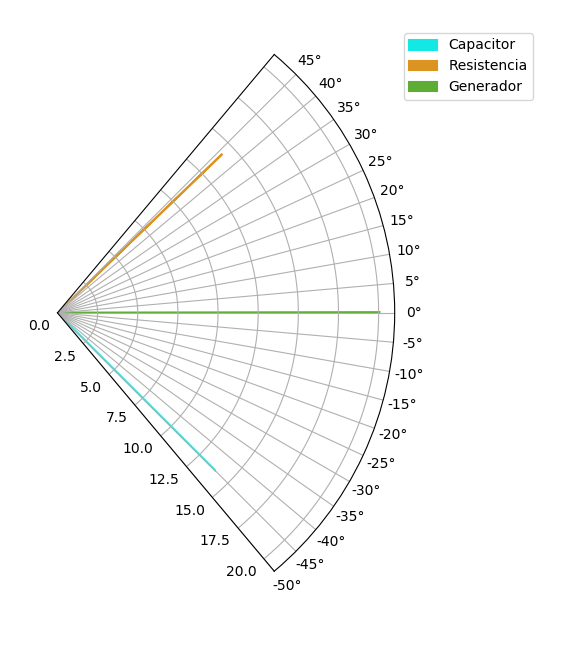
\includegraphics[scale=0.55]{../Desarrollo/diagrama_vectorial.png}
	\end{center}
	\caption{Diagrama vectorial de tensiones, donde la del generador es la resultante de la suma}
\end{figure}

\subsubsection*{Respuesta en frecuencia}

En este apartado se busca obtener la respuesta en frecuencia del circuito filtro pasabajos de manera pr\'actica, midiendo la respuesta del circuito a una se\~nal senoidal de amplitud $20V$ para cada frecuencia, tanto en m\'odulo como en fase y graficarlo en una escala semilogar\'itmica. Adem\'as, se contrastar\'a el resultado de tales mediciones con lo obtenido te\'oricamente. En la figura  se dibuja con un trazo el bode de magnitud te\'orico y con puntos los valores del mismo medidos en la pr\'actica.

En la tabla de mediciones de bode, hay algunas mediciones de la fase medida con el m\'etodo XY que no pudieron ser completadas dado que en la forma obtenida no era distinguible la distancia entre cruce de ceros.

\begin{table}[H]
	\centering
	\begin{tabular}{c c c c c c c c c c}%
		$\bm{f}$ & $\bm{v_{g}}$ & $\bm{v_{c}}$ & $\bm{\frac{V_c}{V_g}db}$ & $\bm{\theta_{osc}}$ & $\bm{\delta_{T}}$ & $\bm{\theta_{T}}$ & $\bm{\delta_{cero}}$ & $\bm{\delta_{total}}$ & $\bm{\theta_{xy}}$ \\ \hline
		\csvreader[head to column names, late after line=\\]{../Mediciones/Excel/bode_modulo_capacitor.csv}{}{\frec & \vg & \vc & \h & \osc & \delta & \tiempo & \ceros & \total & \xy}
		\hline
	\end{tabular}
	\label{mediciones_bode}
	\caption{Mediciones del m\'odulo de la respuesta en frecuencia}
\end{table}

\begin{figure}[H]
	\begin{center}
		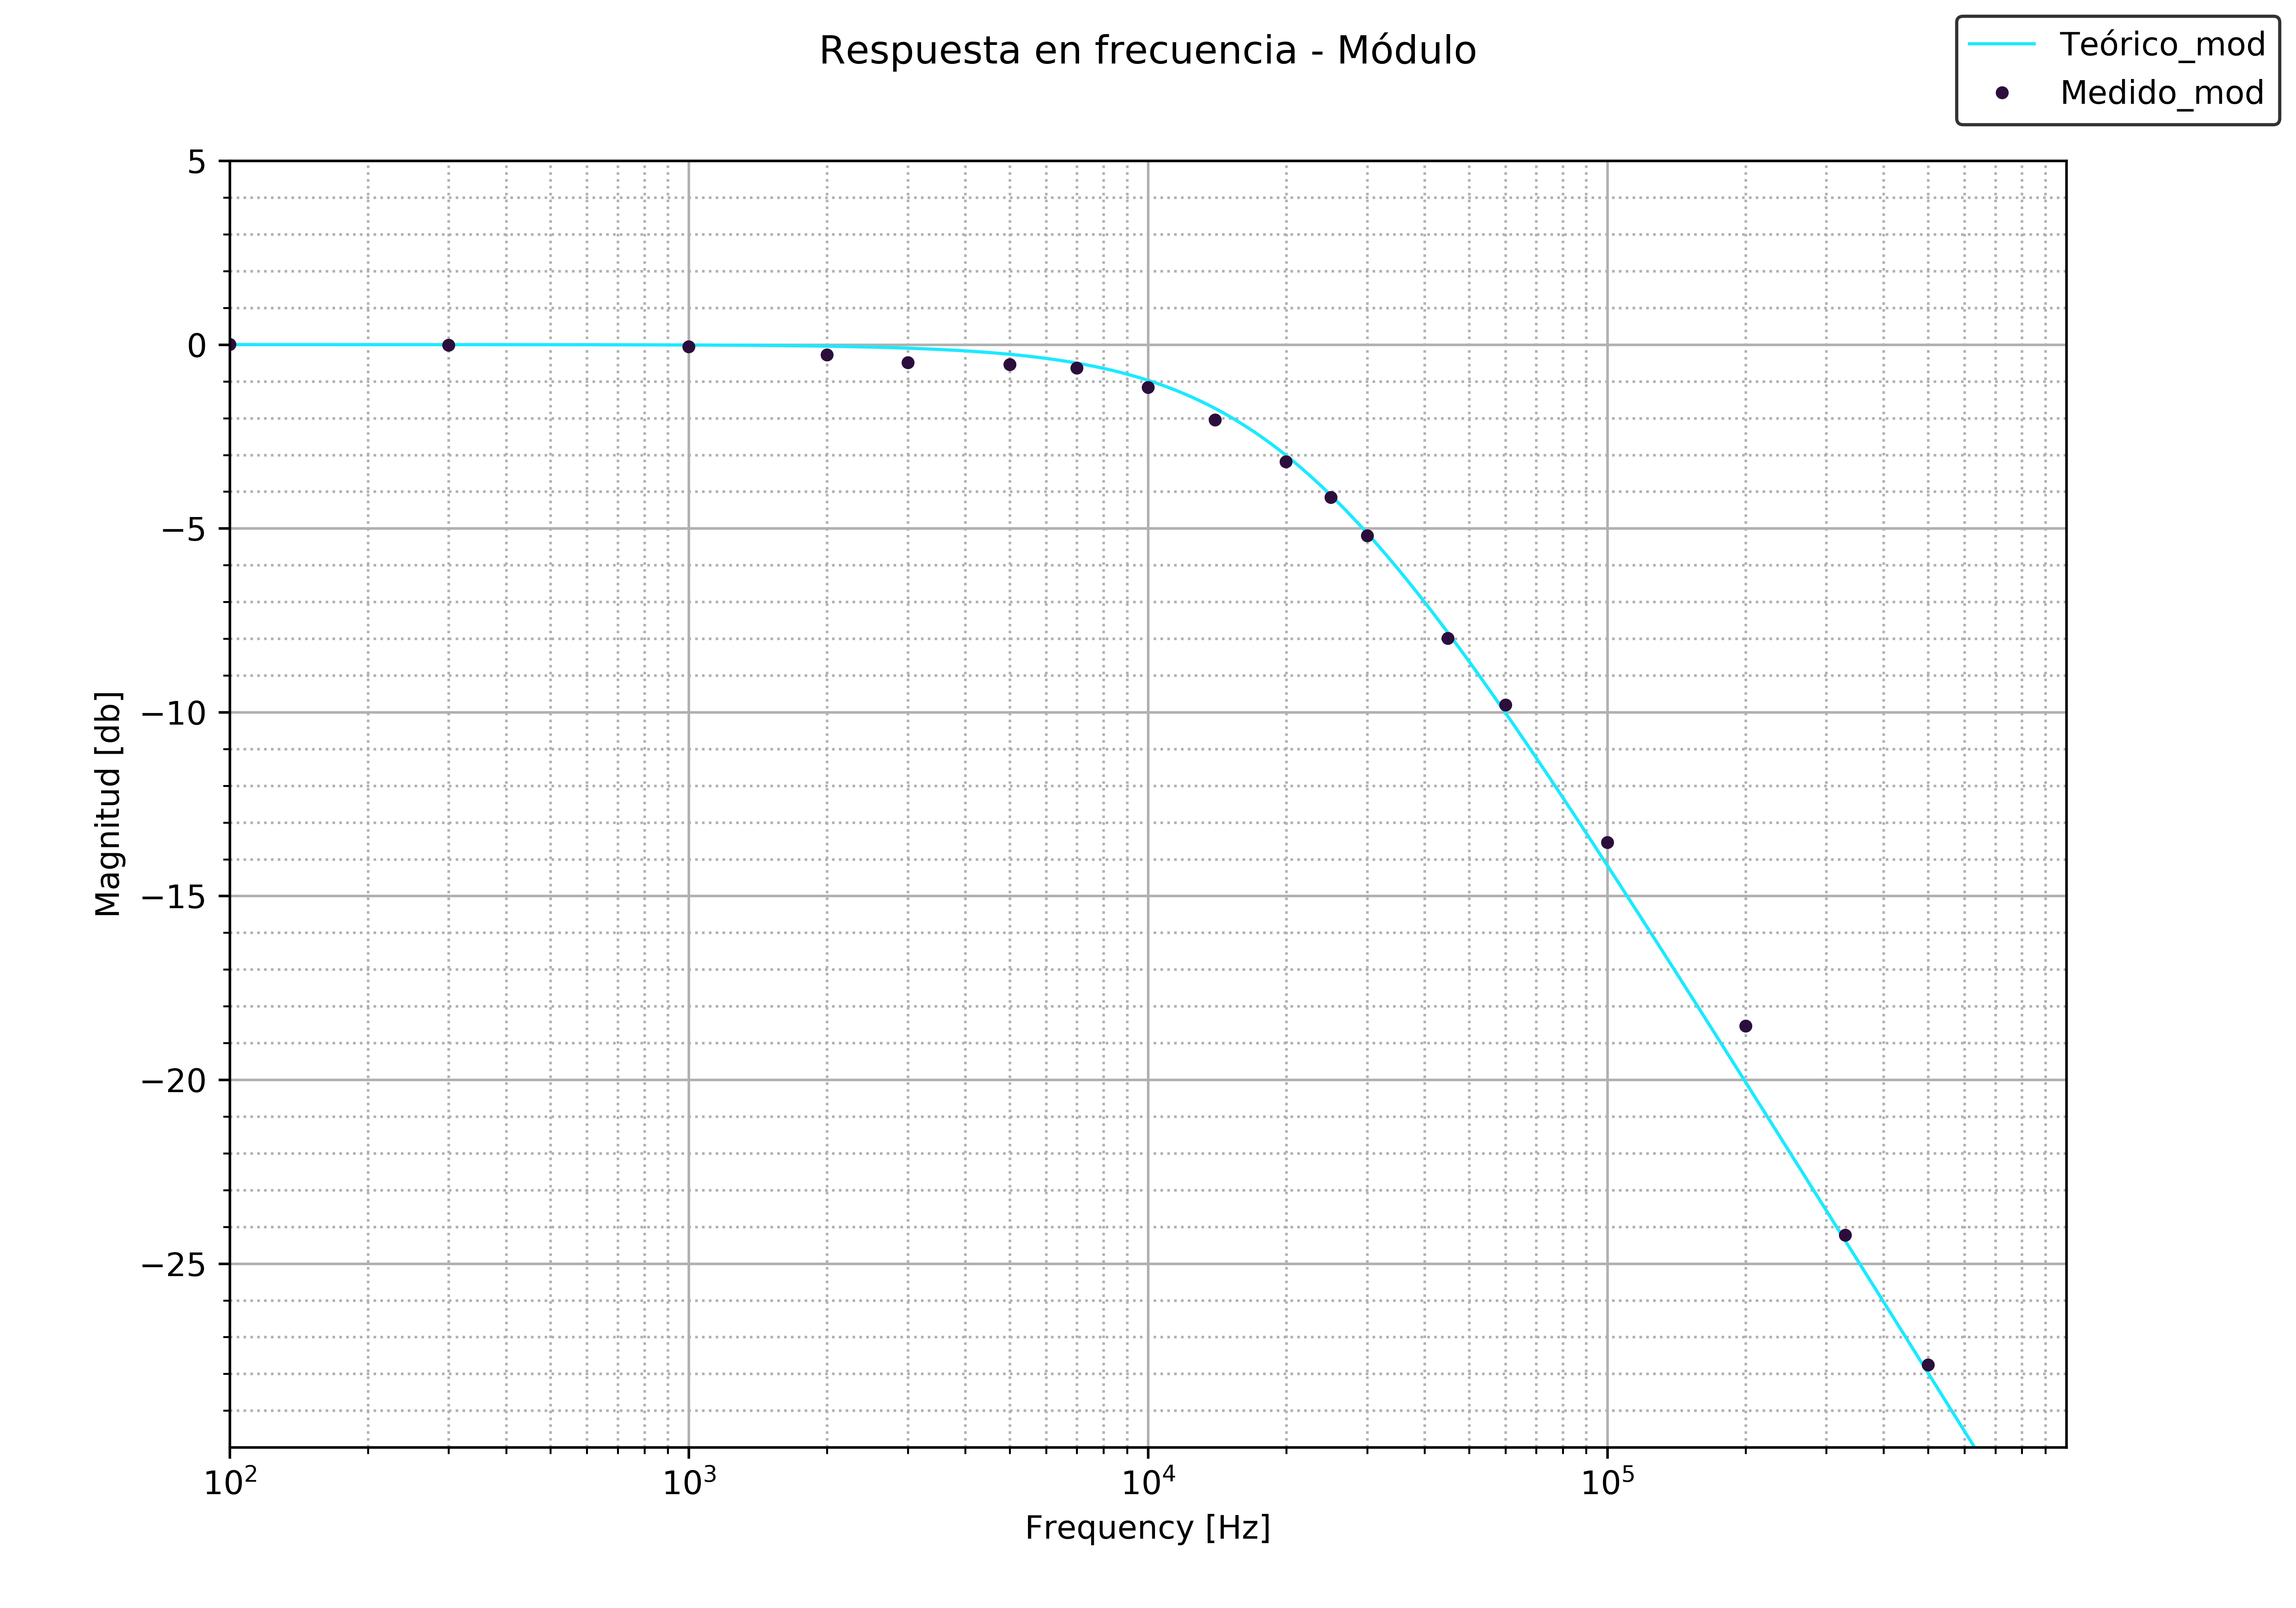
\includegraphics[scale=0.6]{../Desarrollo/bode_modulo.png}
	\end{center}
	\caption{Diagrama de bode de m\'odulo}
	\label{fig:bode_modulo}
\end{figure}

\begin{figure}[H]
	\begin{center}
		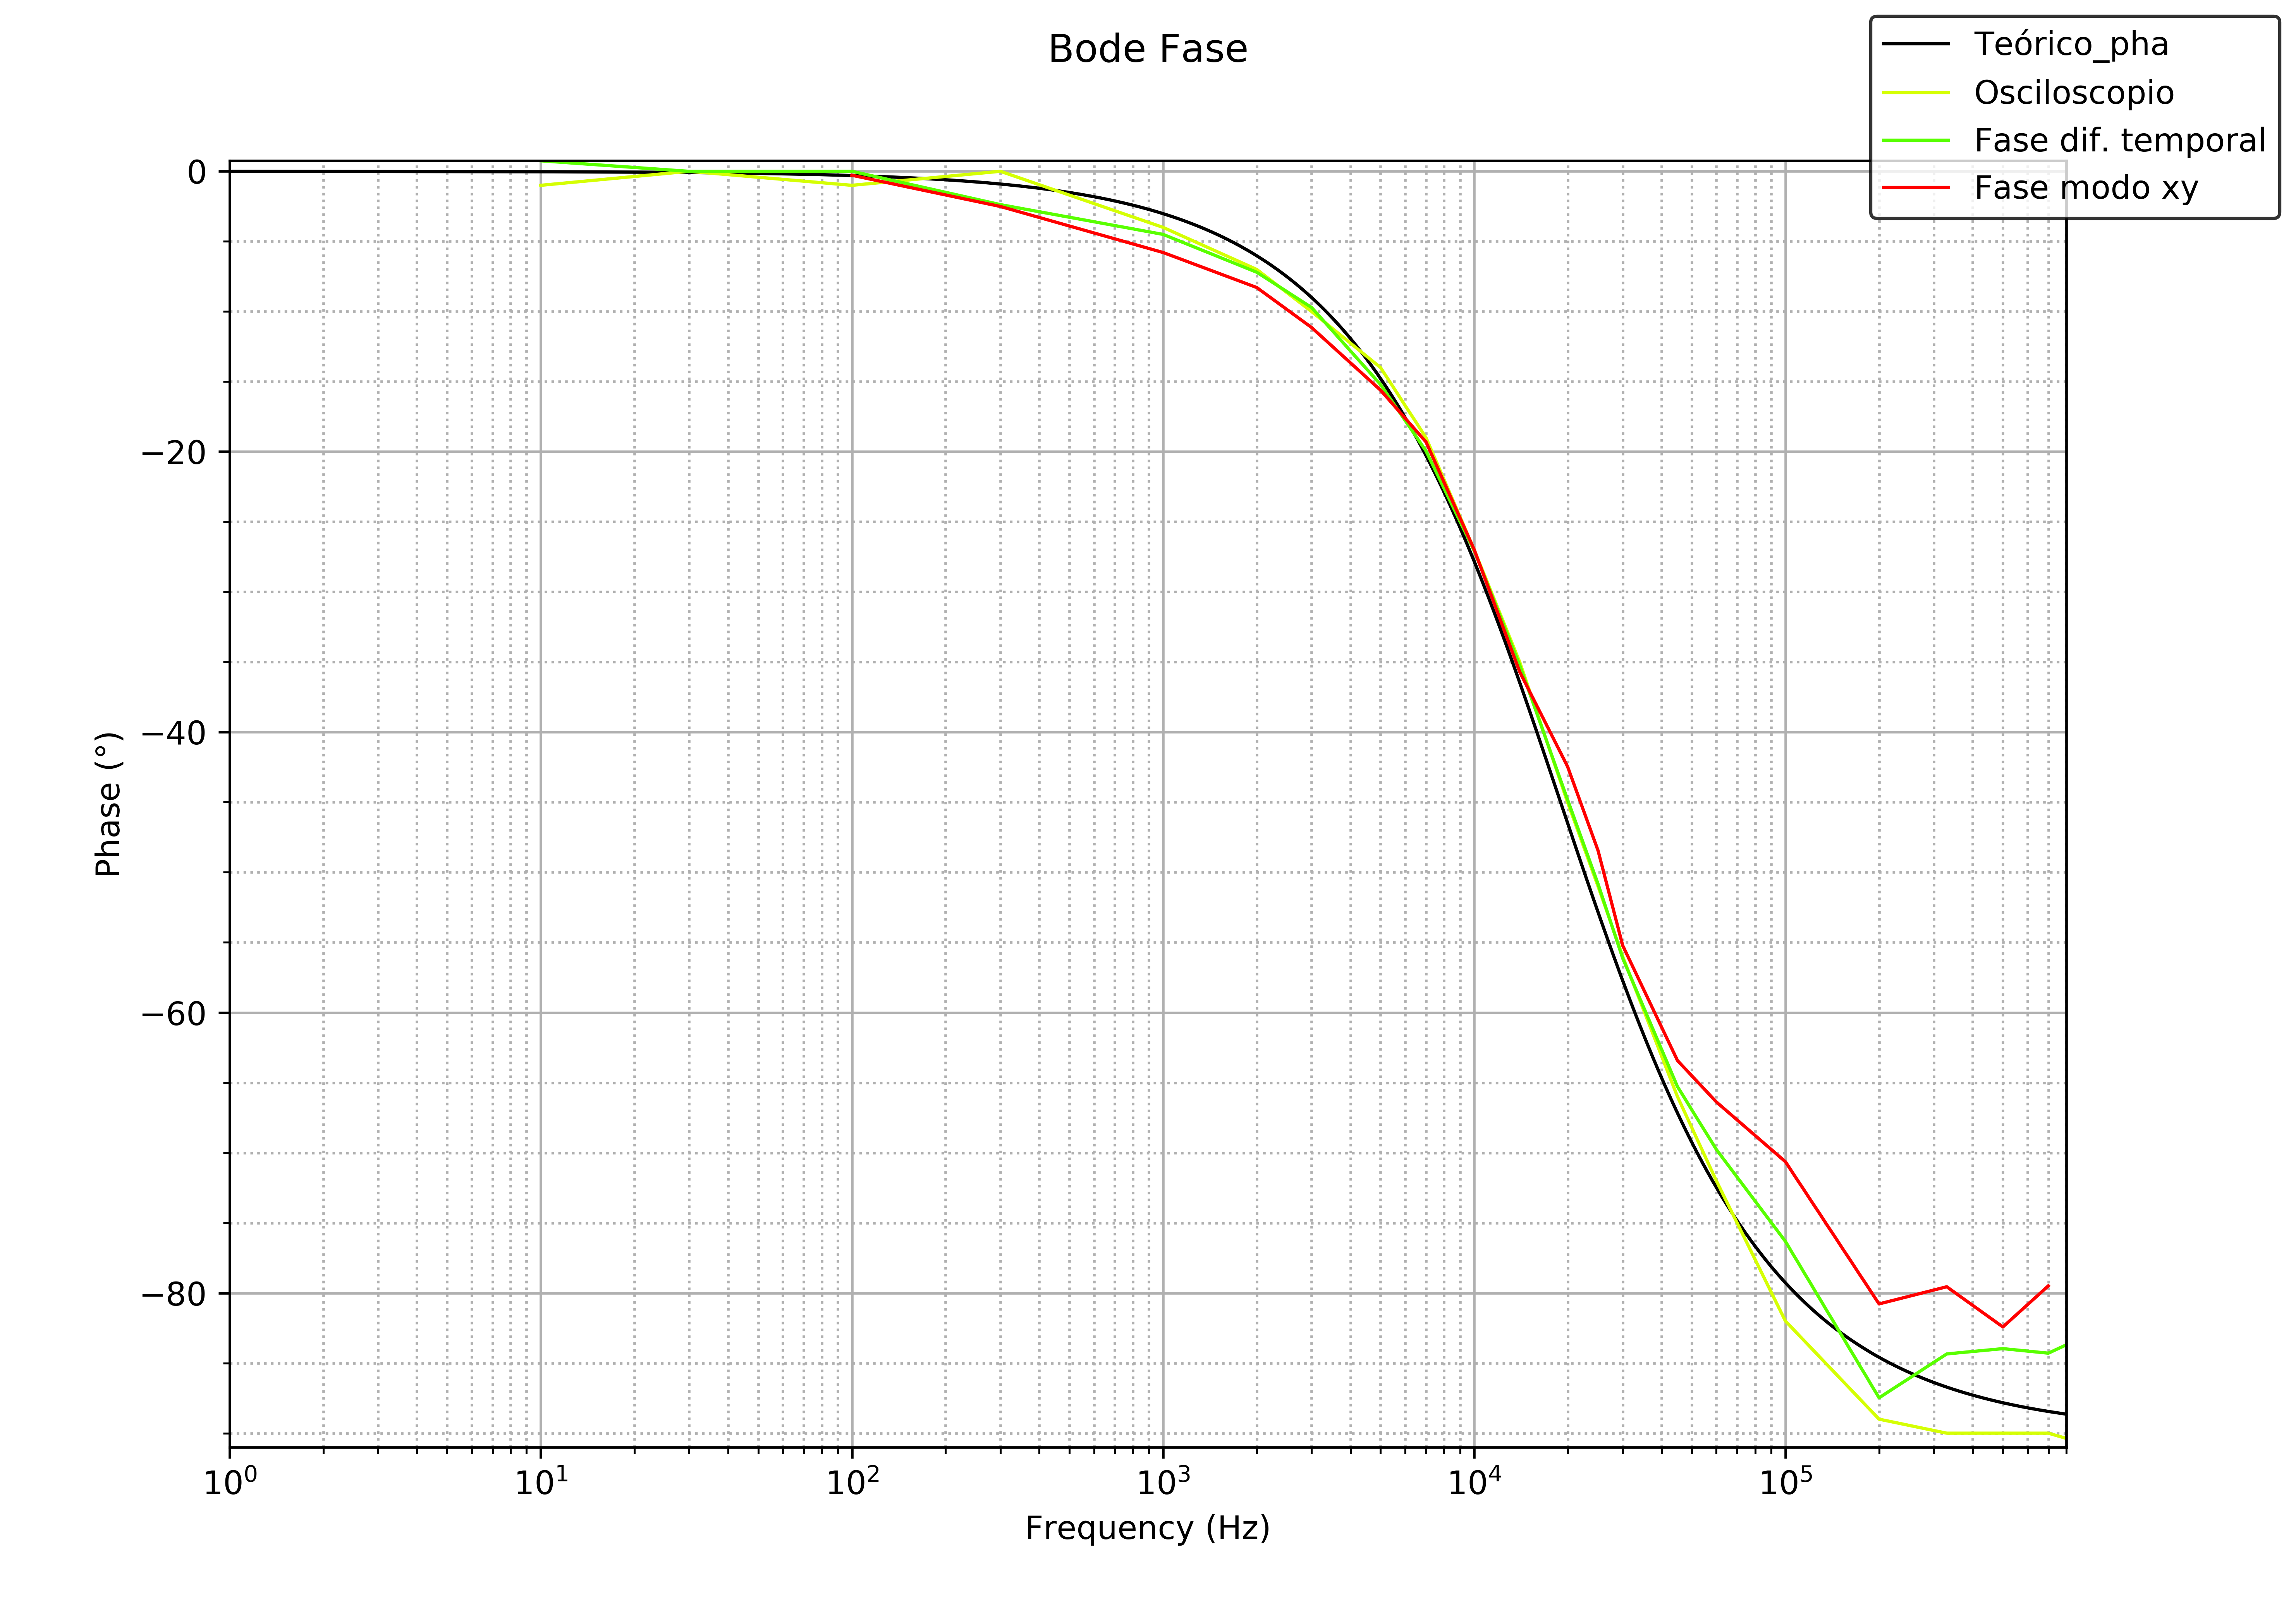
\includegraphics[scale=0.6]{../Desarrollo/bode_fase.png}
	\end{center}
	\caption{Diagrama de bode de fase}
	\label{fig:bode_fase}
\end{figure}

\subsubsection*{Amplitud de resistencia en frecuencia}

En el circuito RC, para poder medir la amplitud sobre la resistencia se necesita medir las amplitudes de las se\~nales sobre el generador y sobre el capacitor y emplear la herramiento de resta de math en el osciloscopio. Una vez obtenido eso, se calcula para cada frecuencia el valor de la amplitud y se obtiene el gr\'afico de la figura \ref{fig:amplitud_resistencia}. En tal figura, lo que se puede observar es el comportamiento de un filtro pasa altos, ya que para frecuencias bajas la amplitud de la misma se ve reducida, mientras que para valores muy grandes de frecuencia la atenuaci\'on es casi nula. Es decir, la resistencia en este circuito posee un comportamiento inverso al del capacitor.

\begin{table}[H]
	\centering
	\begin{tabular}{c c}%
		$\bm{f}$ & $\bm{v_{r}}$ \\ \hline
		\csvreader[head to column names, late after line=\\]{../Mediciones/Excel/resistencia.csv}{}{\frec & \vr}
		\hline
	\end{tabular}
\end{table}

\begin{figure}[H]
	\begin{center}
		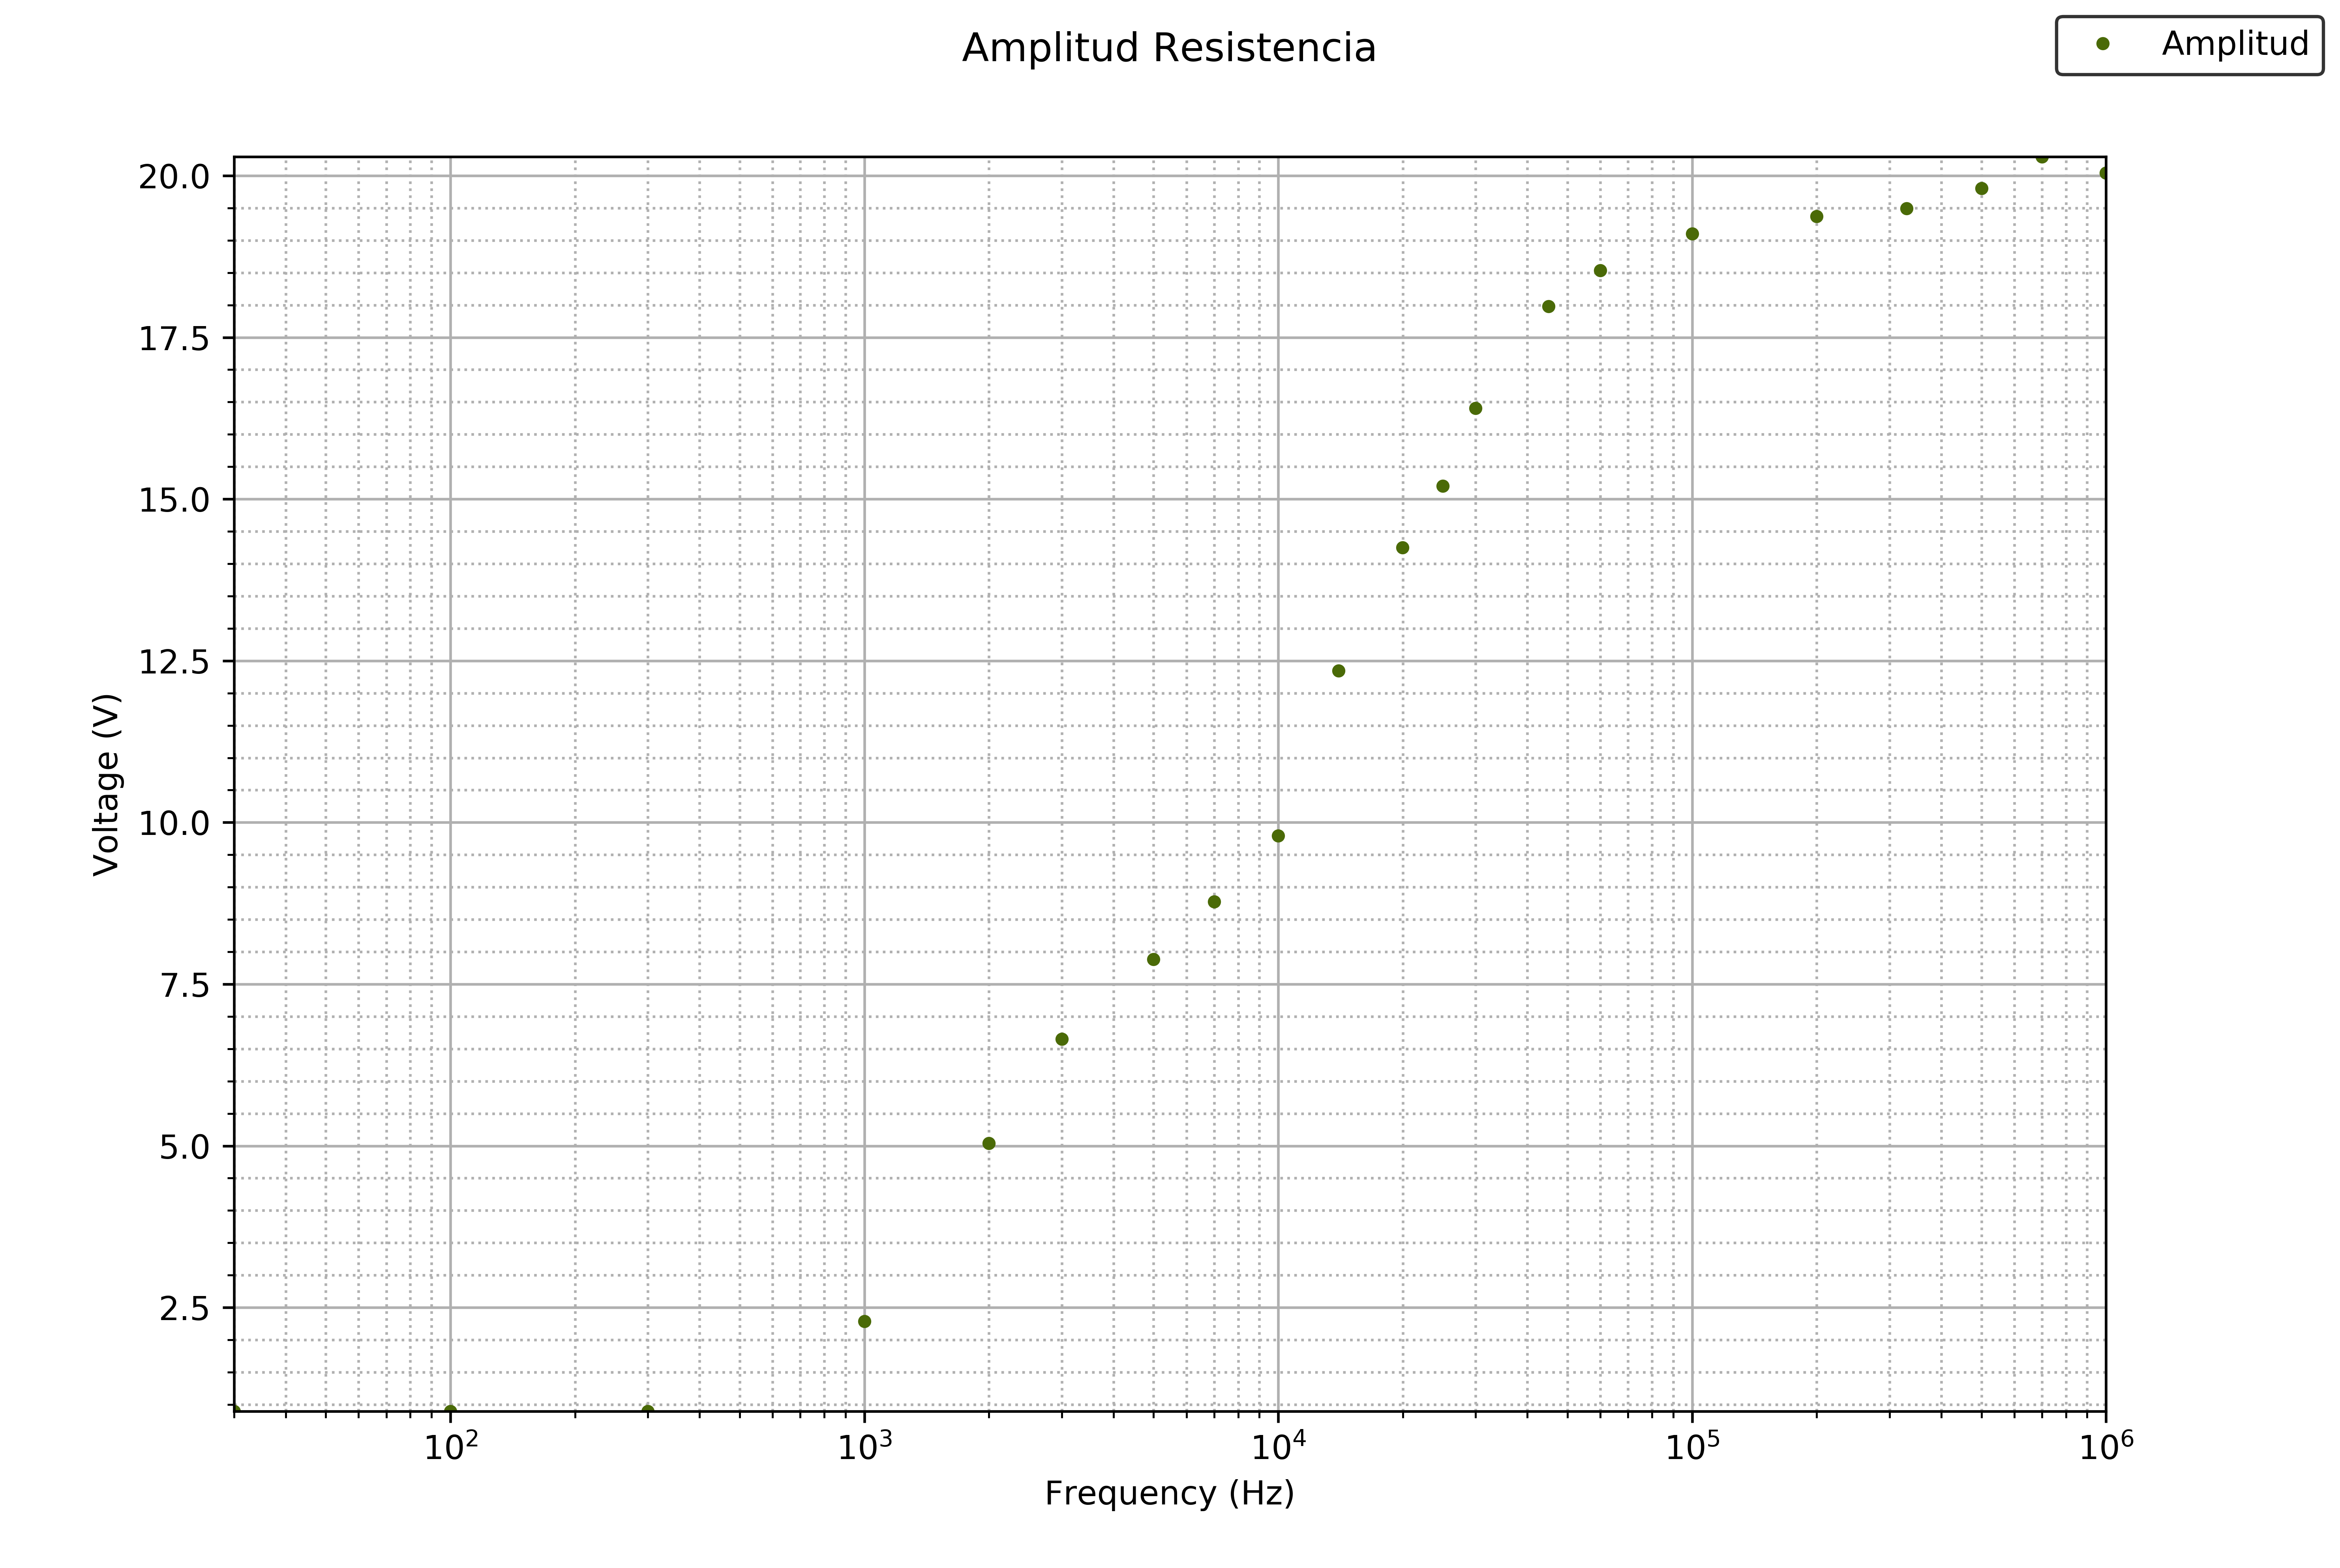
\includegraphics[scale=0.65]{../Desarrollo/amplitud_resistencia.png}
		\caption{Amplitud de la resistencia en funci\'on de la frecuencia}
		\label{fig:amplitud_resistencia}
	\end{center}
\end{figure}

\subsubsection*{Comportamiento frente a se\~nal cuadrada}

En la expresi\'on de la ecuaci\'on \ref{eq:transfer} se puede observar que dada la frecuencia de corte $\omega_o = 18,94kHz$ luego se observa que, desde un punto de vista te\'orico:

\begin{equation}
	H(s) = \frac{1}{1 + \frac{s}{2 \pi \cdot 18,94kHz}}
\end{equation}

Esto mismo da la idea que para frecuencias tales que $f > 189,4kHz$ o m\'as, se puede empezar a aproximar que la funci\'on de transferencia se reduce de la forma:

\begin{equation}
	H(s) = \frac{1}{1 + \frac{s}{2 \pi \cdot 18,94kHz}} \Rightarrow
	H(s) \approx \frac{1}{\frac{s}{2 \pi \cdot 18,94kHz}}
\end{equation}

Por la propiedad de la integral para la transformada de Laplace, se puede observar que dividir por la variable compleja $s$ consiste en integral la funci\'on o se\~nal en el dominio temporal. Desde otro punto de vista, la antitransformada de esta funci\'on es el escal\'on, y cualquier se\~nal de salida puede obtenerse a partir de la convoluci\'on con la respuesta impulsiva lo cual, dado que es un escal\'on, se reduce en una integral sobre la entrada.

Desde un an\'alisis en frecuencias, la descomposici\'on en serie de Fourier de la se\~nal cuadrada dar\'ia como resultado que est\'a compuesta por infinitas componentes arm\'onicas de frecuencias m\'ultiplo de la fundamental, lo cual al momento de pasar a trav\'es del filtro pasabajo conduce a que algunas de las frecuencias m\'as altas se vean atenuadas, deformando la forma de onda original.

En las figuras ilustradas, se puede observar que ante una se\~nal de entrada cuadrada, las respuestas del circuito var\'ian seg\'un la frecuencia de la cuadrada, y finalmente, para frecuencias muy altas la salida es la integral de la entrada.

\begin{tabular}{c c}
	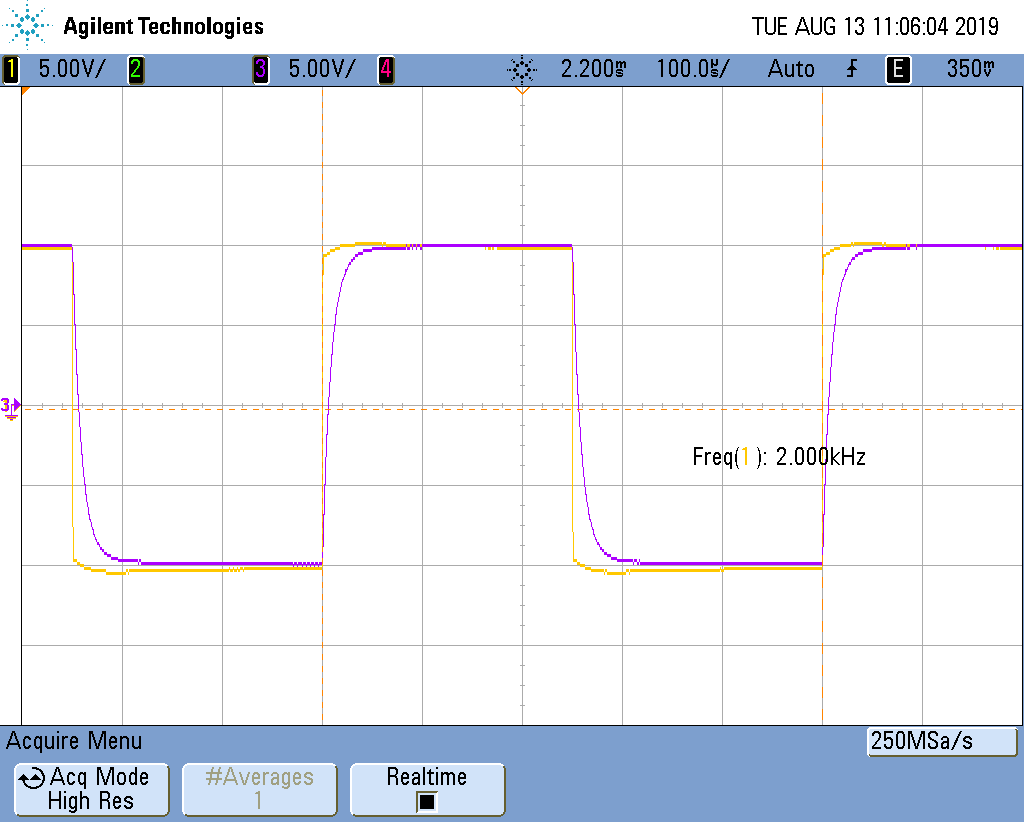
\includegraphics[scale=0.21]{../Mediciones/Fotos/scope_4.png} & 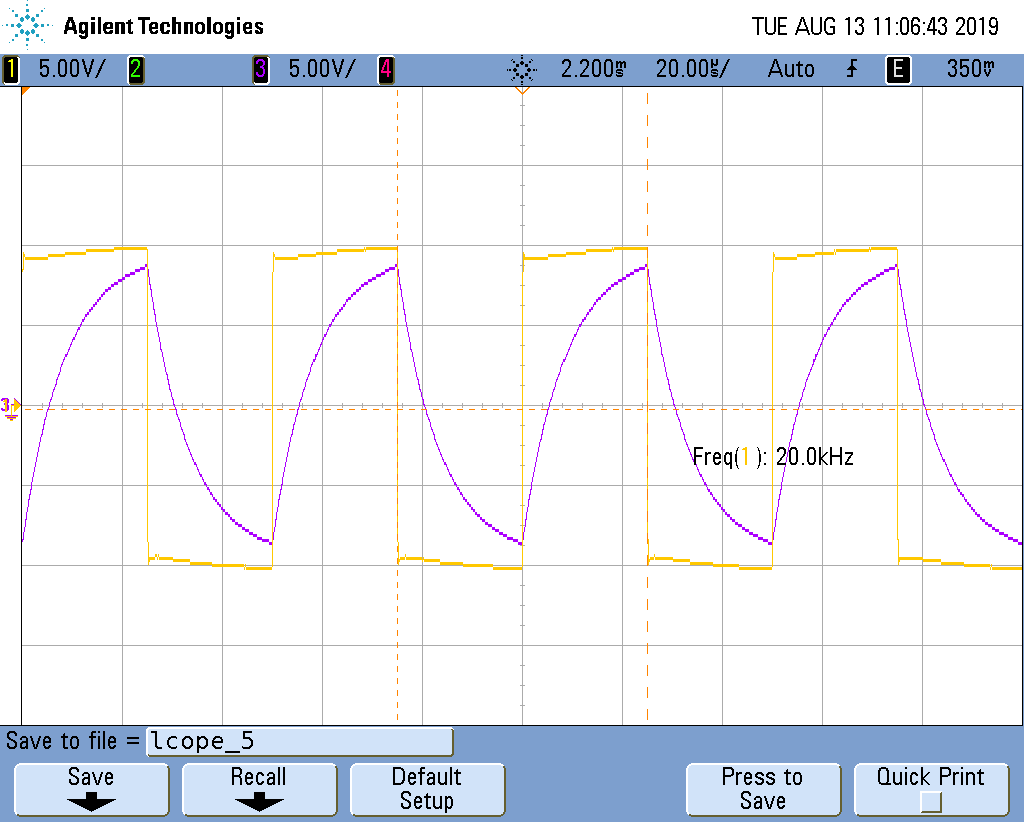
\includegraphics[scale=0.21]{../Mediciones/Fotos/scope_5.png}	\\
	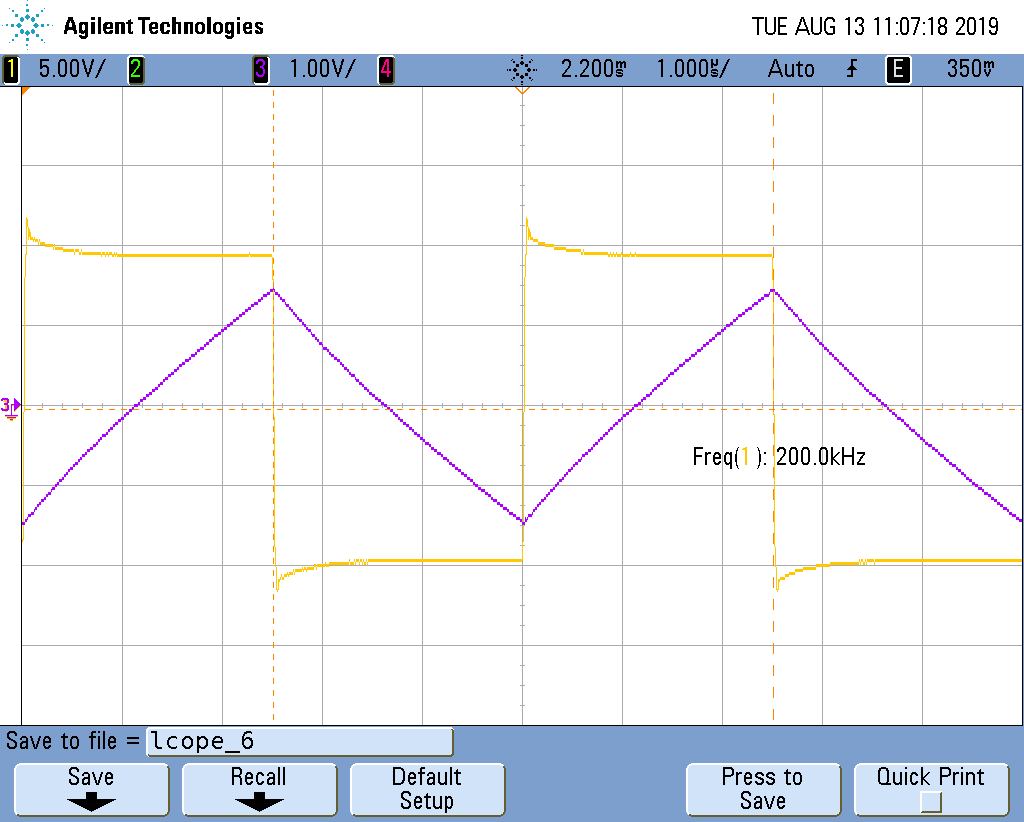
\includegraphics[scale=0.21]{../Mediciones/Fotos/scope_6.png} & 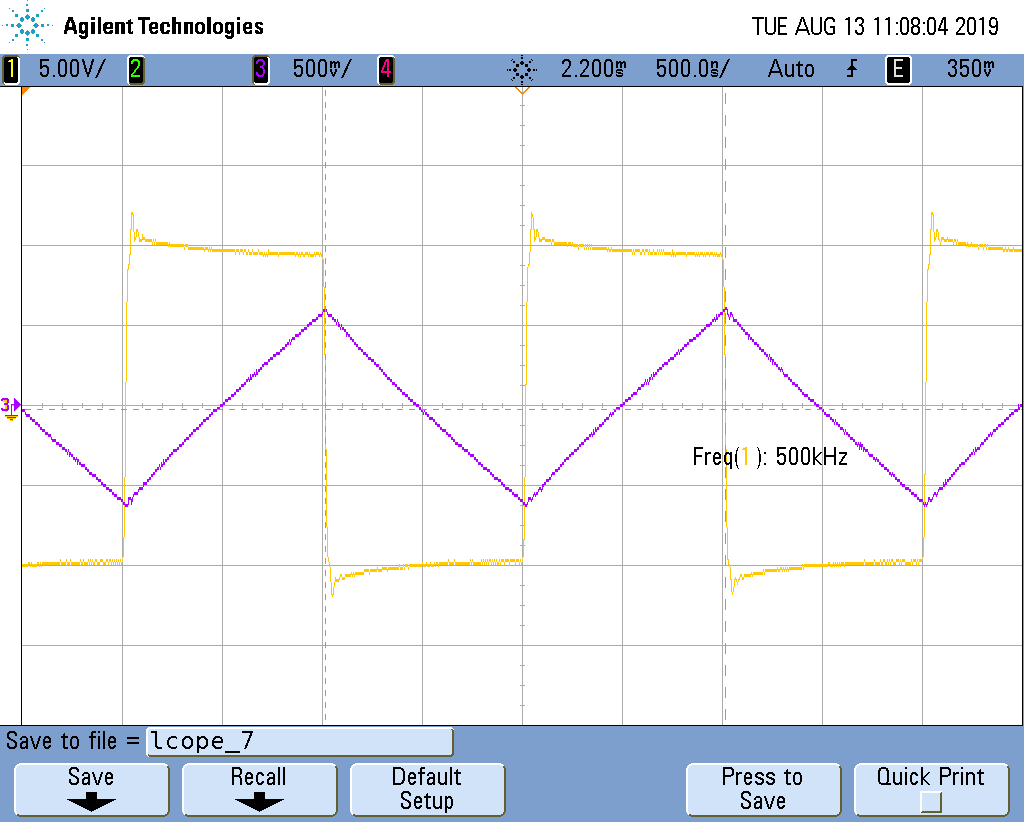
\includegraphics[scale=0.21]{../Mediciones/Fotos/scope_7.png}	
\end{tabular}

\subsubsection*{Reemplazando capacitor por punta de osciloscopio}

En este apartado se arma el circuito pero quitando el capacitor de la salida, midiendo con la punta del osciloscopio, pues se conoce el modelo de tal punta y contiene un capacitor que es el que determinar\'a la frecuencia de corte del filtro. De esta forma se buscan las frecuencias de corte para los escenarios en los cuales la punta se encuentre configurada en x1 y en x10, y se contrasta el valor resultante de capacidad con el medido por el analizador de impedancias a la misma frecuencia.

\begin{table}[H]
	\centering
	\caption{Medici\'on de frecuencia de corte en x1}
	\begin{tabular}{c c c c}
		$V_{gen}$ & $f_{gen}$ & $|V_{cap}|$ & $\phase{V_{cap}}$ \\
		\hline
		$18,9V$ & $250kHz$ & $13,4V$ & $-45^{\circ}$		
	\end{tabular}
\end{table}

\begin{table}[H]
	\centering
	\caption{Comparaci\'on de capacidades calculada y medida en x1}
	\begin{tabular}{c c c c c}
		$f_{corte}$ & $R$ & $C_{calc}$ & $C_{med}$ & $Error(\%)$ \\
		\hline
		$250kHz$ & $5,6k \Omega$ & $113,68 \cdot 10^{-12}$ & $116,6 \cdot 10^{-12}$ & $2,5$ \\
		$250kHz$ & $5,46k \Omega$ & $116,59 \cdot 10^{-12}$ & $116,6 \cdot 10^{-12}$ & $0,002$
	\end{tabular}
\end{table}

\begin{table}[H]
	\centering
	\caption{Medici\'on de frecuencia de corte en x10}
	\begin{tabular}{c c c c}
		$V_{gen}$ & $f_{gen}$ & $|V_{cap}|$ & $\phase{V_{cap}}$ \\
		\hline
		$19,98V$ & $1,4MHz$ & $13,92V$ & $-45^{\circ}$		
	\end{tabular}
\end{table}

\begin{table}[H]
	\centering
	\caption{Comparaci\'on de capacidades calculada y medida en x10}
	\begin{tabular}{c c c c c}
		$f_{corte}$ & $R$ & $C_{calc}$ & $C_{med}$ & $Error(\%)$ \\
		\hline
		$1,4MHz$ & $5,6k \Omega$ & $20,30 \cdot 10^{-12}$ & $17,1 \cdot 10^{-12}$ & $18,72$ \\
		$1,4MHz$ & $5,46k \Omega$ & $20,82 \cdot 10^{-12}$ & $17,1 \cdot 10^{-12}$ & $21,76$
	\end{tabular}
\end{table}

\subsection{Análisis de resultados}

Con respecto a las capacidades e impedancias medidas al comienzo, puede decirse que la variaci\'on de los valores nominales de los componentes frente a los comerciales dentro del margen impuesto por la tolerancia suele tener una incidencia considerable sobre los resultados obtenidos. Para poder medir esta incidencia se utilizó el analizador de impedancias y modelando al capacitor con una resistencia en paralelo se calculó una frecuencia de corte real mayor a la teórica. Luego, con éstos mismos valores se midió la amplitud de la señal de salida con diferentes métodos obteniendose asi gráficos para al fase y el módulo. Tanto de la figura \ref{fig:bode_modulo} como de la figura \ref{fig:bode_fase} puede verse que los datos teóricos y los medidos por el osciloscopio concuerdan con un pequeño error a altas frecuencias. A medida que aumenta la frecuencia este error se hace mayor, ya que las impedancias de los componentes comienzan a cambiar llegado este punto. A pesar de lo anterior, consideramos que son necesarias más mediciones para poder determinar el comportamiento exacto del circuito a altas frecuencias. Por otro lado, Los datos medidos mediante el modo XY poseen mayor desviación, debido a que éste es un método aproximado que depende de la resolución de la pantalla para ser medido. 


Con respecto al comportamiento del circuito frente a una señal cuadrada, pudo mostrarse gráfica y teóricamente como afecta un filtro pasabajos a dicho tipo de señal. Se concluye entonces, que a frecuencias mucho mayores a la frecuencia de corte, llamese uno o mas órdenes de magnitud mayor, el circuito se comporta como un integrador. No es el mejor integrador posible, ya que depende de la frecuencia de corte del circuito y de que tan lejos se trabaje de la misma.


Finalmente pudo comprobarse la capacidad introducida al circuito cuando se utiliza una punta de osciloscopio. Se logró medir dicha capacidad y así demostrar que el solo hecho de tomar una medición implica modificar la misma.

